Development of SIM started with development in phases which focus on particular need of project.
Various phases and their detail are given below -:
\begin{itemize}
\item Phase I (C++) -: \\
	During Phase I, we wrote code in C++ to parse Staad Pro file to the database (Mysql).
\item Phase II (Mysql) -: \\
    During Phase II, we make the schema of Mysql tables in which all the attributes of 
    Staad pro are present. Phase I and II are very much interlinked because C++ code i.e. 
    act as a parser and Mysql used to store the output data of the parser.
\item Phase III (Django) -: \\
    During phase III, we record small macros (interpreted code) in FreeCAD and then transfer that macro
    in the form of class and objects.
\item Phase IV (Django) -: \\
    During phase IV, we provided web interface to this software using Django. Djanog was used
    to get input from user and write some.csv file and after that FreeCAD macro will run
    automatically and give its respectively output in the form of PDF, SVG, .fcstd.
\item Phase V (Rendering 3D model) -: \\
    During phase V, we convert the .fcstd file to WebGL format file to rendering 3D 
    model on the browser screen. Sed command is used for changing the value some 
    constraint.
\item Phase VI (Testing and documentation) -: \\ 
    During final phase, we tested the software for various conditions and then applied required error control and messaging
    mechanism. Also in this phase, we documented the project( developers documentation and README.md) using doxygen and wrote the report for this software.    
\end{itemize}     

\subsection{Upload STAAD.Pro file}
SIM communicates with the database back at the server end and interact to store and retrieve information. A processing of the file is considered complete only if all of the file has been parsed, it database objects has been created by the corresponding function and the objects have been properly transferred to the database at the back end. If this is not the case then no changes shall be made to the database and its consistent state must be maintained.

\begin{figure}[h!]
\begin{center}
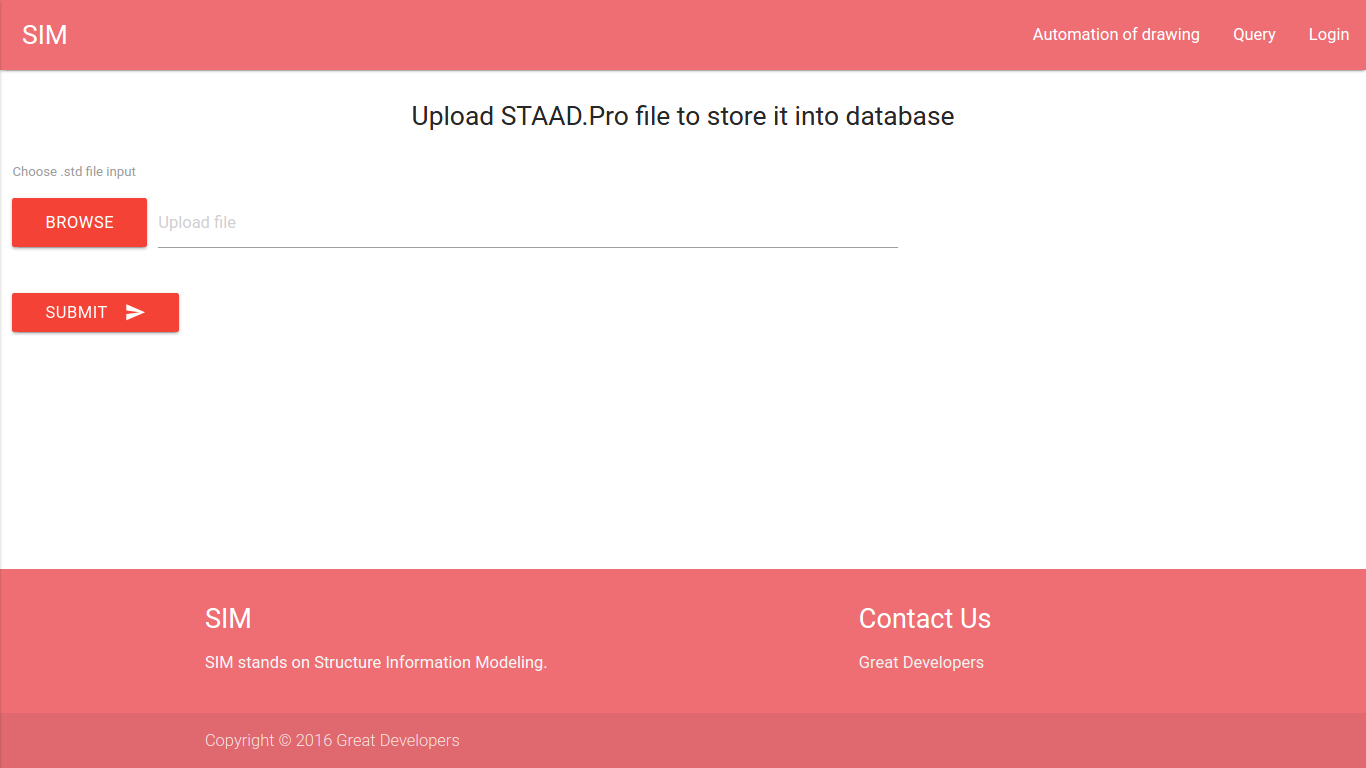
\includegraphics[scale=0.33]{images/sim_index.png}
\label{si}
\caption{Front page}
\end{center}
\end{figure}

If the system recognizes that the file in consideration is not correct then it must point that out to the user and also be able to tell that in what manner is the file wrong. For example, if the file is wrong syntactically then the correct syntactic suggestion must be provided to the user.  If the file is not complete then simply a message must be passed to the user.

\begin{figure}[h!]
\begin{center}
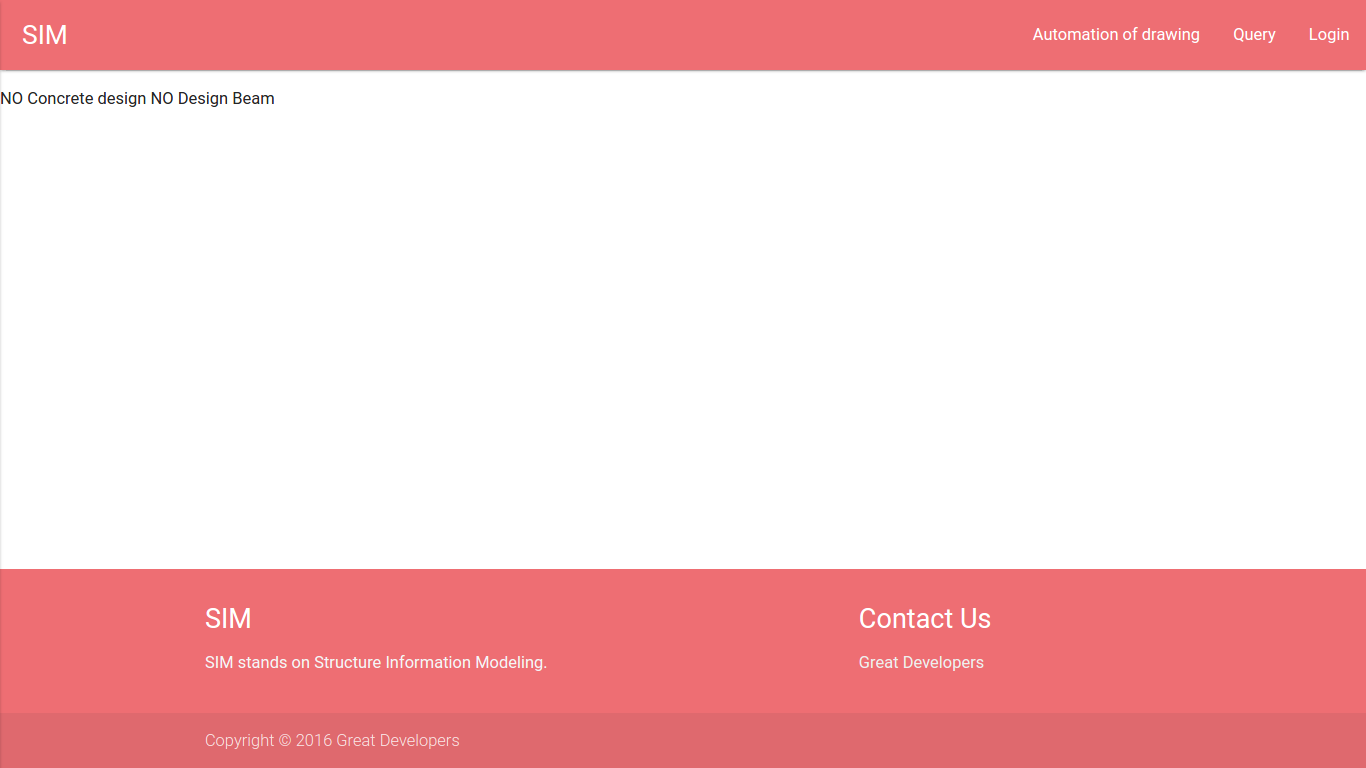
\includegraphics[scale=0.33]{images/after_upload.png}
\caption{Result show on submitted the Staad.Pro file}
\label{si2}  
\end{center}
\end{figure}
\newpage
\subsection{Query}
The user must be able to apply queries on the information stored in the databases.
All the data stored in the database is shown in the tabular form with all the fields that are related to the respective element as shown in Fig \ref{si3}.

\begin{figure}[h!]
\begin{center}
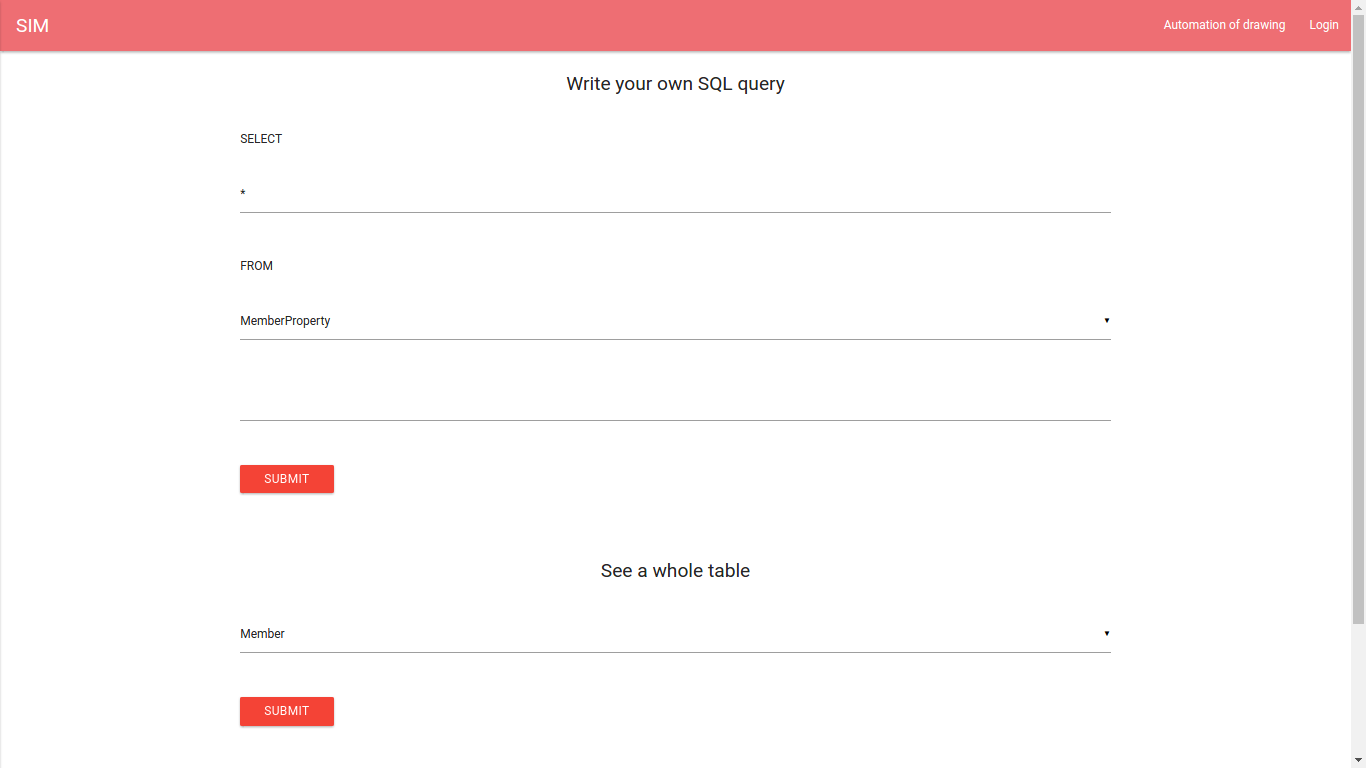
\includegraphics[scale=0.33]{images/query.png}
\caption{Query page}
\label{si3}  
\end{center}
\end{figure}

Result of the query is shown Fig. \ref{si4}.

\begin{figure}[h!]
\begin{center}
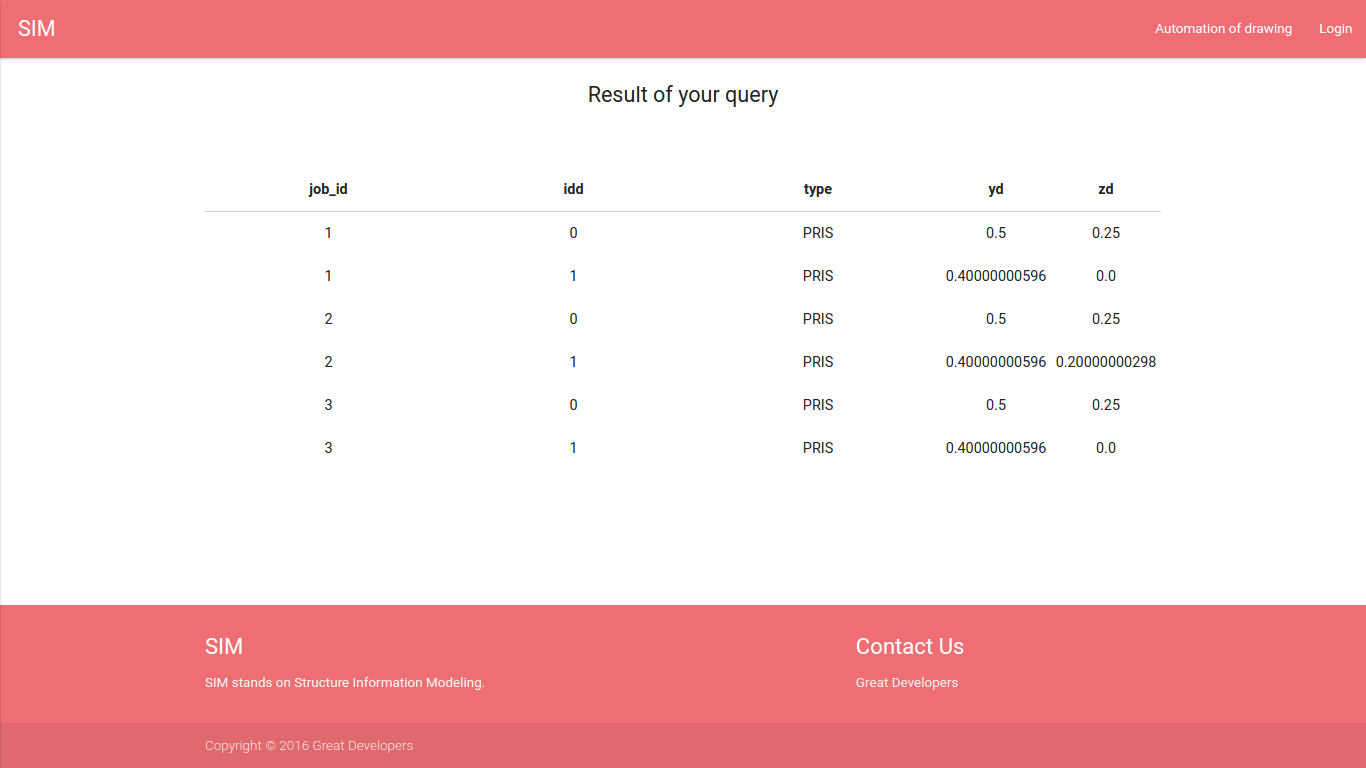
\includegraphics[scale=0.33]{images/result_query.png}
\caption{Result of query}
\label{si4}  
\end{center}
\end{figure}

\subsection{Automation of Drawings}
\subsubsection{Enter Building specifications}
The user makes the drawings of different views of the building on the
drawing sheets. The user will be able to enter the specifications of the building through the web
browser (Fig. \ref{si5}) and on the back-end, the FreeCAD macros will use those input values to draw the drawings of different views of the building on different drawing
sheets. The output of the same can then be taken by a user in SVG, PDF and fcstd formats.

\begin{figure}[h!]
\begin{center}
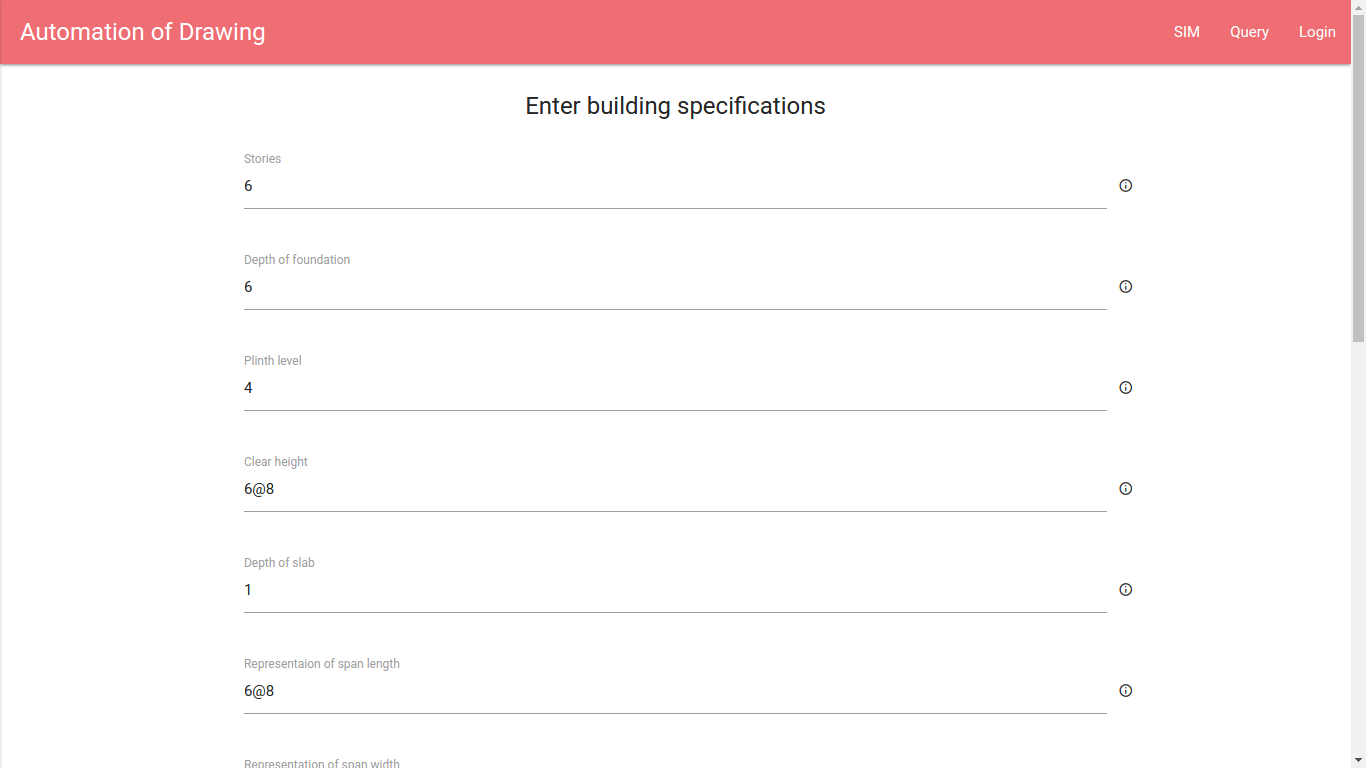
\includegraphics[scale=0.35]{images/auto_drawing.png}
\caption{Form to enter the specifications of the building}
\label{si5}  
\end{center}
\end{figure}

\subsubsection{Download project as zip}
After submitting the form this page will redirect to download page(Fig. 3.6). Here the user will see all the submitted value of in form (Fig. \ref{si6}) and download its project.
\begin{figure}[h!]
\begin{center}
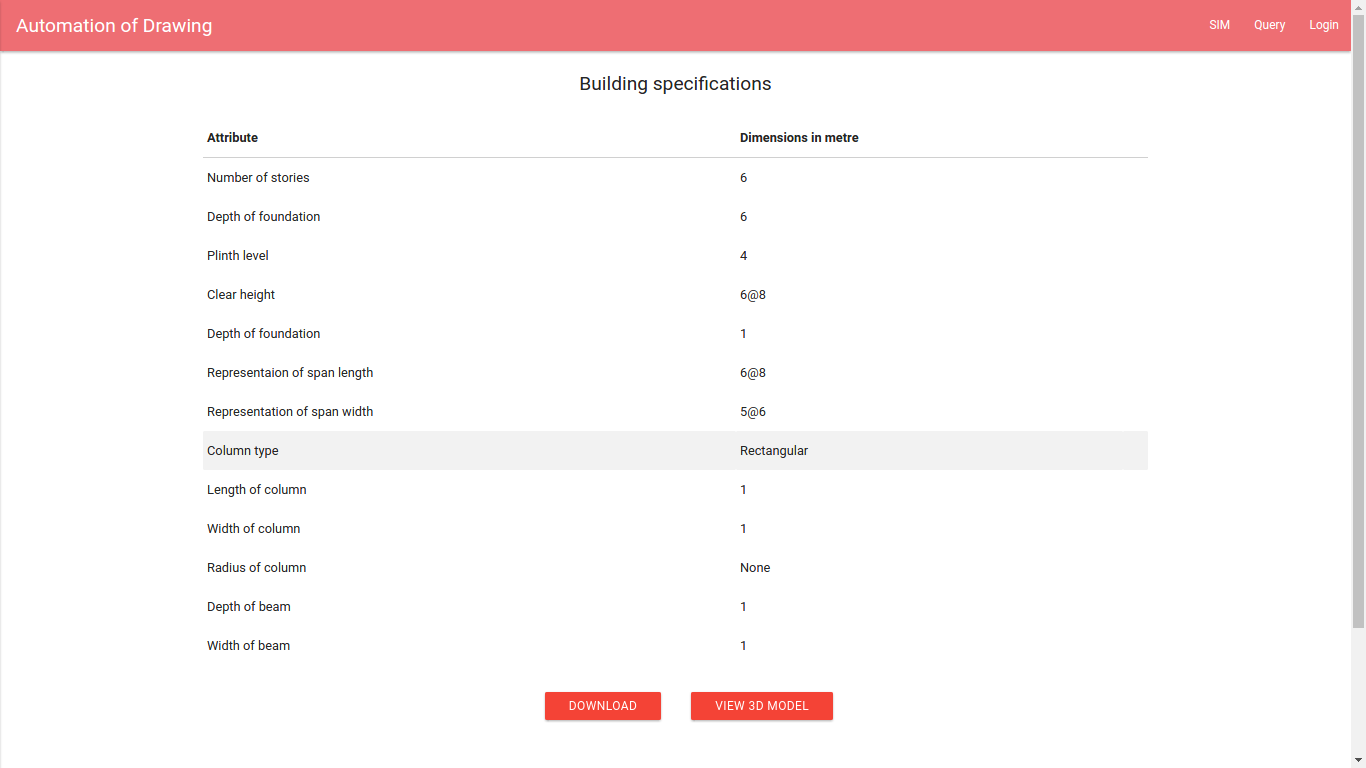
\includegraphics[scale=0.35]{images/b_specs.png}
\caption{Form to enter the specifications of the building}
\label{si6}  
\end{center}
\end{figure}
The zip file will contain different views (like side view, front view, a top view and many sectional views according to the building stories) of the building in PDF as well in SVG format. It also contains .fcstd file (FreeCAD project file) Fig. \ref{si7}. By using .fcstd file the user will modify the existing project and can perform a wide range of operations.

\begin{figure}[h!]
\begin{center}
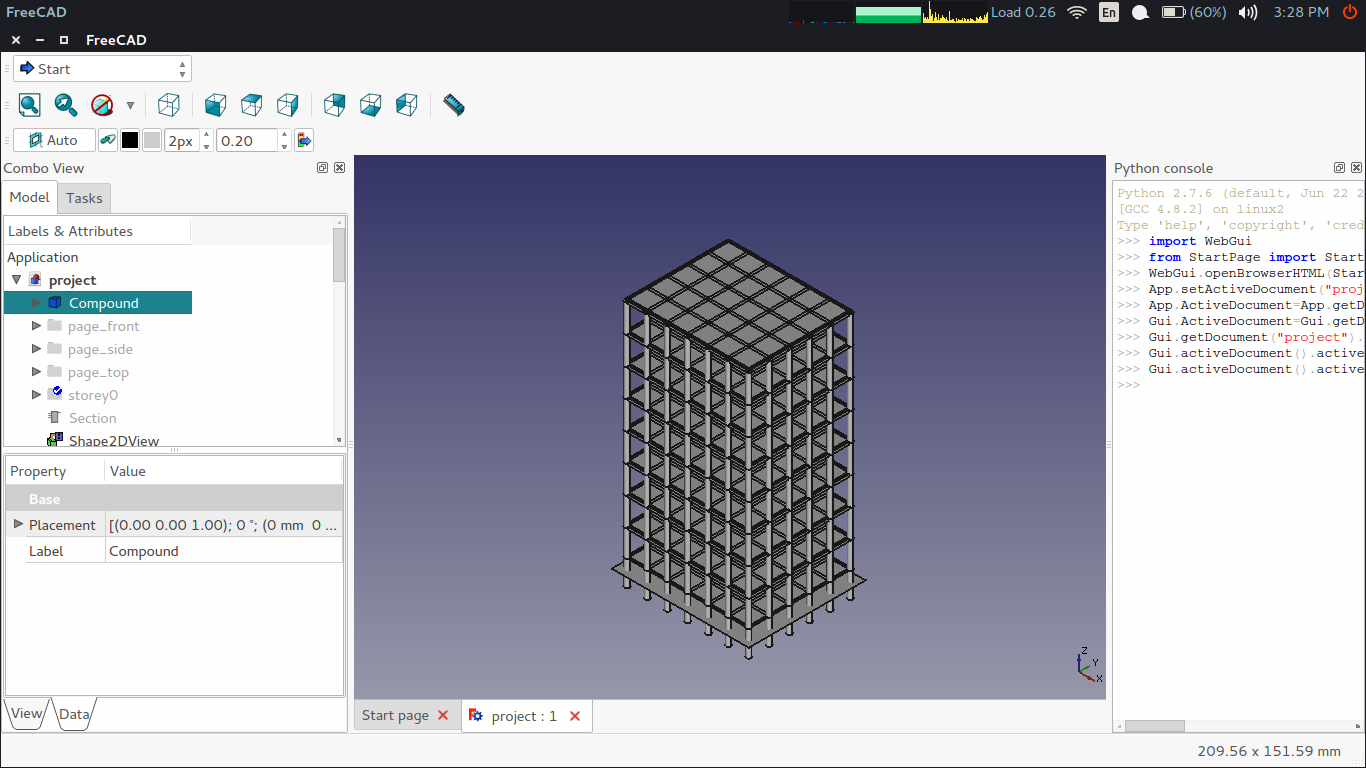
\includegraphics[scale=0.35]{images/building_macro.png}
\caption{Opening .fcstd file in FreeCAD}
\label{si7}  
\end{center}
\end{figure}

\subsubsection{View 3D model}
This feature will render the 3D model of the building on the browser screen. In this process, FreeCAD exporter convert .fcstd file to WebGL format (Web Graphics Library is a JavaScript API for rendering interactive 3D and 2D graphics within any compatible web browser without the use of plug-ins).   

\begin{figure}[h!]                                                      
\begin{center}                                                          
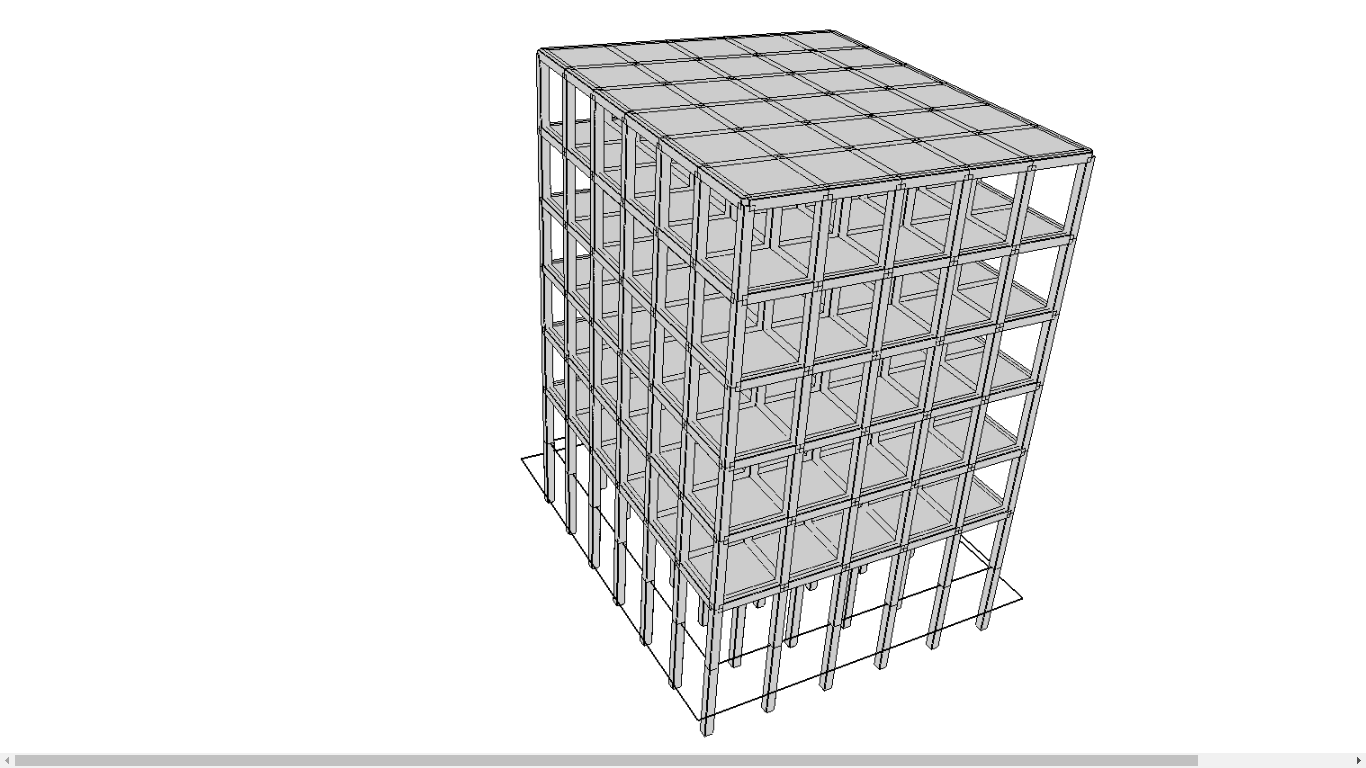
\includegraphics[scale=0.35]{images/3dmodel.png}                        
\caption{Admin page}              
\end{center}                                                            
\end{figure} 

\section{Adminstration Login}
One of the most powerful parts of SIM is the admin interface Fig . It reads metadata from your models to provide a quick, model-centric interface where trusted users can manage content on your site. The admin’s recommended use is limited to an organisation’s internal management tool. It’s not intended for building your entire front end around.

\begin{figure}[h!]                                                      
\begin{center}                                                          
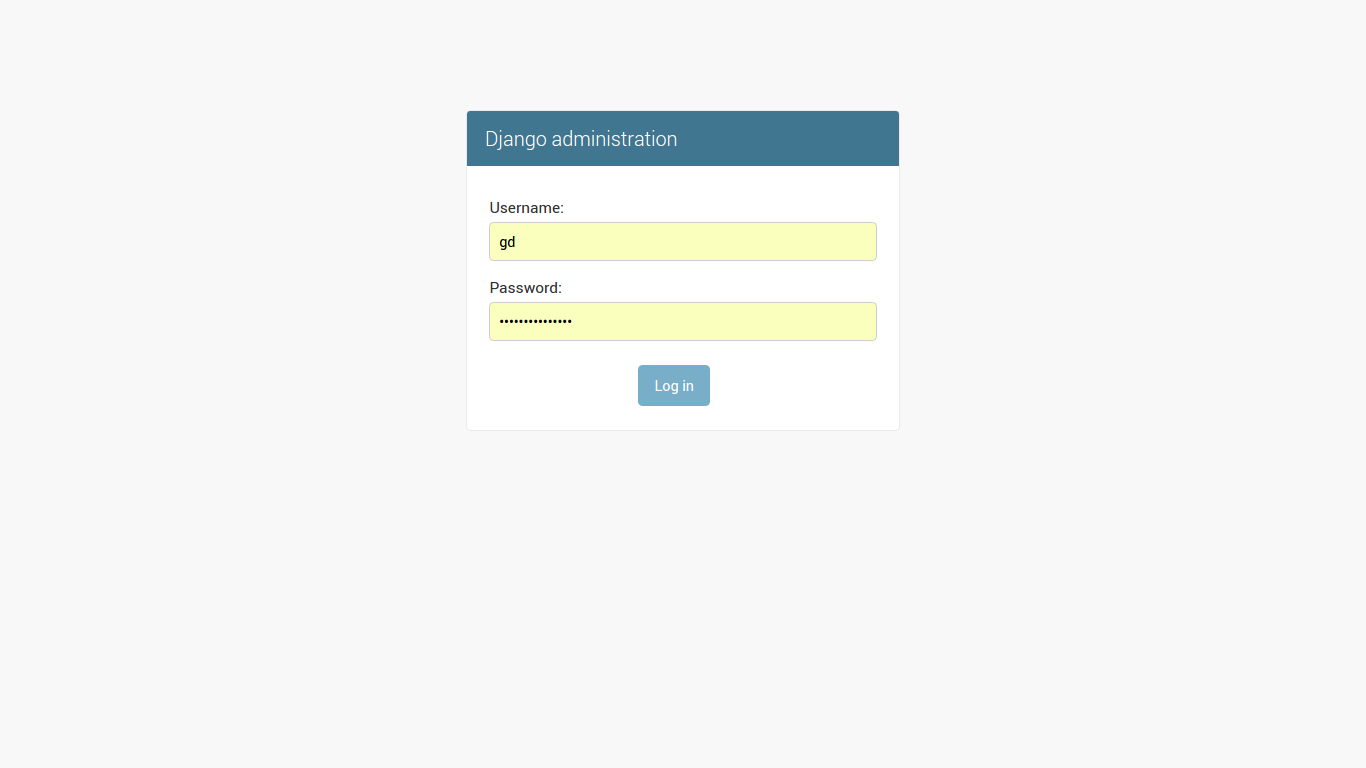
\includegraphics[scale=0.35]{images/admin.png}                        
\caption{Login page}                            
\end{center}                                                            
\end{figure} 

The admin has many hooks for customization, but beware of trying to use those hooks exclusively. If you need to provide a more process-centric interface that abstracts away the implementation details of database tables and fields, then it’s probably time to write your own views.

\begin{figure}[h!]                                                      
\begin{center}                                                          
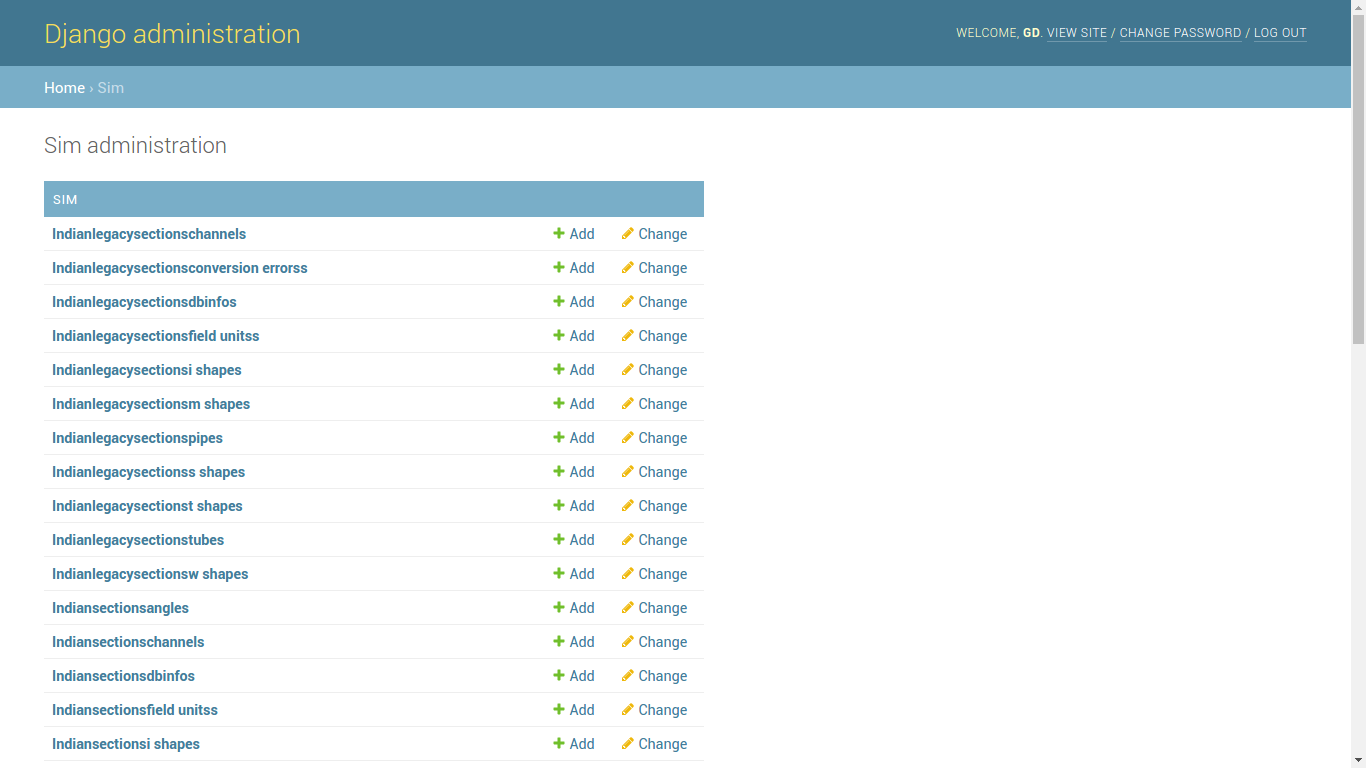
\includegraphics[scale=0.35]{images/admin2.png}                        
\caption{Entities of Staad Pro}                            
\end{center}                                                            
\end{figure} 

\begin{figure}[h!]                                                      
\begin{center}                                                          
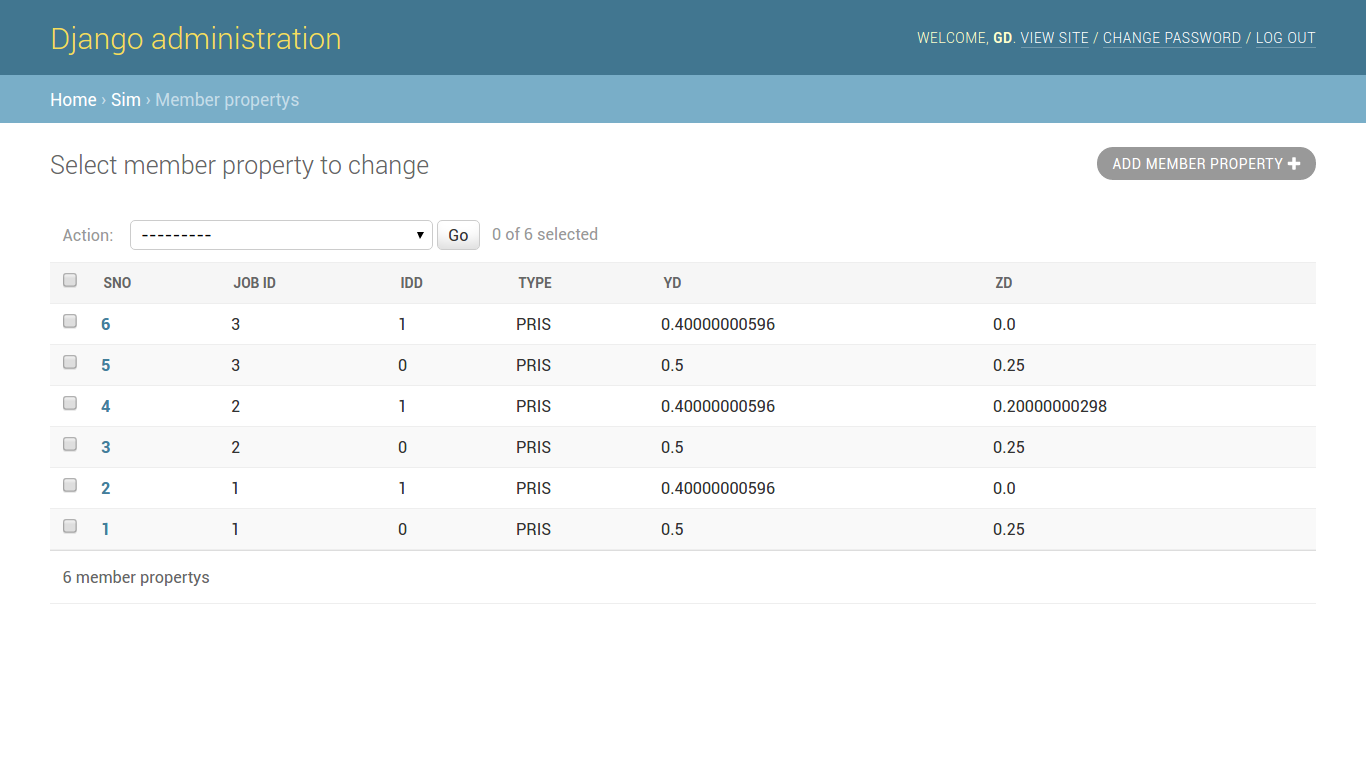
\includegraphics[scale=0.35]{images/admin3.png}                        
\caption{Attributes of each entity}                            
\end{center}                                                            
\end{figure} 

\begin{figure}[h!]                                                      
\begin{center}                                                          
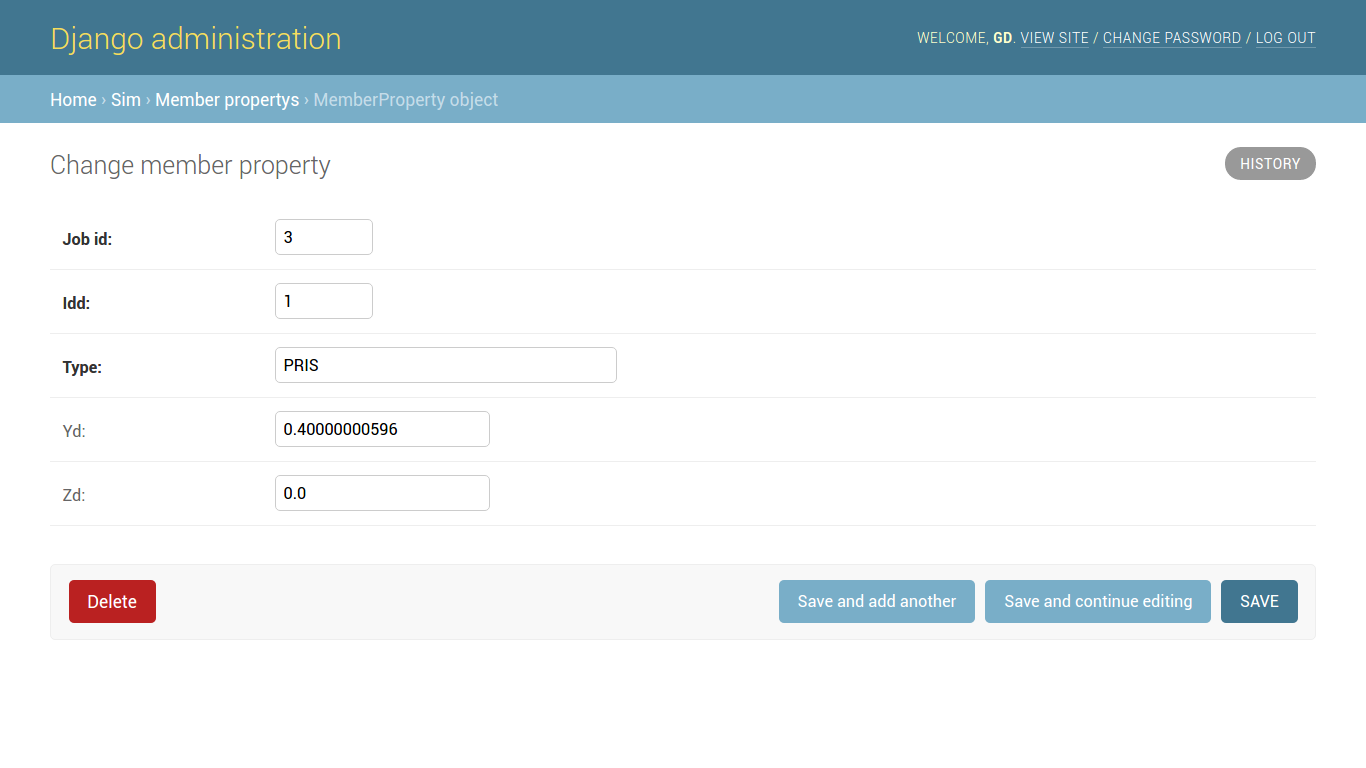
\includegraphics[scale=0.35]{images/admin4.png}                        
\caption{Modification, creation and deleting entity}                            
\end{center}                                                            
\end{figure} 
